%
% General structure for the revdetua class:
%
\documentclass[...]{revdetua}
\usepackage{graphicx}

%
% Valid options are:
%
%   longpaper --------- \part and \tableofcontents defined
%   shortpaper -------- \part and \tableofcontents not defined (default)
%
%   english ----------- main language is English (default)
%   portugues --------- main language is Portuguese
%
%   draft ------------- draft version
%   final ------------- final version (default)
%
%   times ------------- use times (postscript) fonts for text
%
%   mirror ------------ prints a mirror image of the paper (with dvips)
%
%   visiblelabels ----- \SL, \SN, \SP, \EL, \EN, etc. defined
%   invisiblelabels --- \SL, \SN, \SP, \EL, \EN, etc. not defined (default)
%
% Note: the final version should use the times fonts
% Note: the really final version should also use the mirror option
%

\begin{document}

\Header{1}{25}{outubro}{2022}{0}
% Note: the month must be in Portuguese

\title{Finding the Minimum Weighted Closure of a Graph using Exhaustive Search and a Greedy Algorithm}
\author{Eduardo Santos, nºmec 93107, eduardosantoshf@ua.pt} % or \author{... \and ...}
\maketitle

\begin{abstract}
The objective of this assignment was to find a minimum weighted closure for a given vertex-weighted directed graph \textit{G(V, E)}, with \textit{n} vertices and \textit{m} edges. Exhaustive Search and a Greedy Algorithms were used to solve this problem, with the solution explained in this paper, with both solutions being compared in terms of execution time, as well as complexity. The computations were made using a variety of parameters, which will also be referred on the following sections.
\end{abstract}

\section{Introduction}

A closure of \textit{G} is a set of vertices \textit{C}, such that no edges leave \textit{C}. The weight of a closure is the sum of its vertices’ weights. A \textbf{minimum weight closure} is a closure whose total weight is as small as possible. Both algorithms used computed the minimum weighted closure of a given graph, with each approach and its parameters explained later on.

\section{ Problem Description}

To solve this problem, the first thing to do was to create a random graph, so that it can be used to compute the minimum weighted closure. To do this, the NetworkX Python library was used, which is a very powerful tool when working with the creation, manipulation, and study of the structure, dynamics, and functions of complex networks, or graphs.
To better understand this problem, let's consider a graph with 5 nodes and 5 edges, represented in the figure bellow. In this particular case, and in order to facilitate the explanation, a graph with multiple closures was used. Let's also consider each node's number as its weight. 

\begin{figure}[!htb]
    \centering
    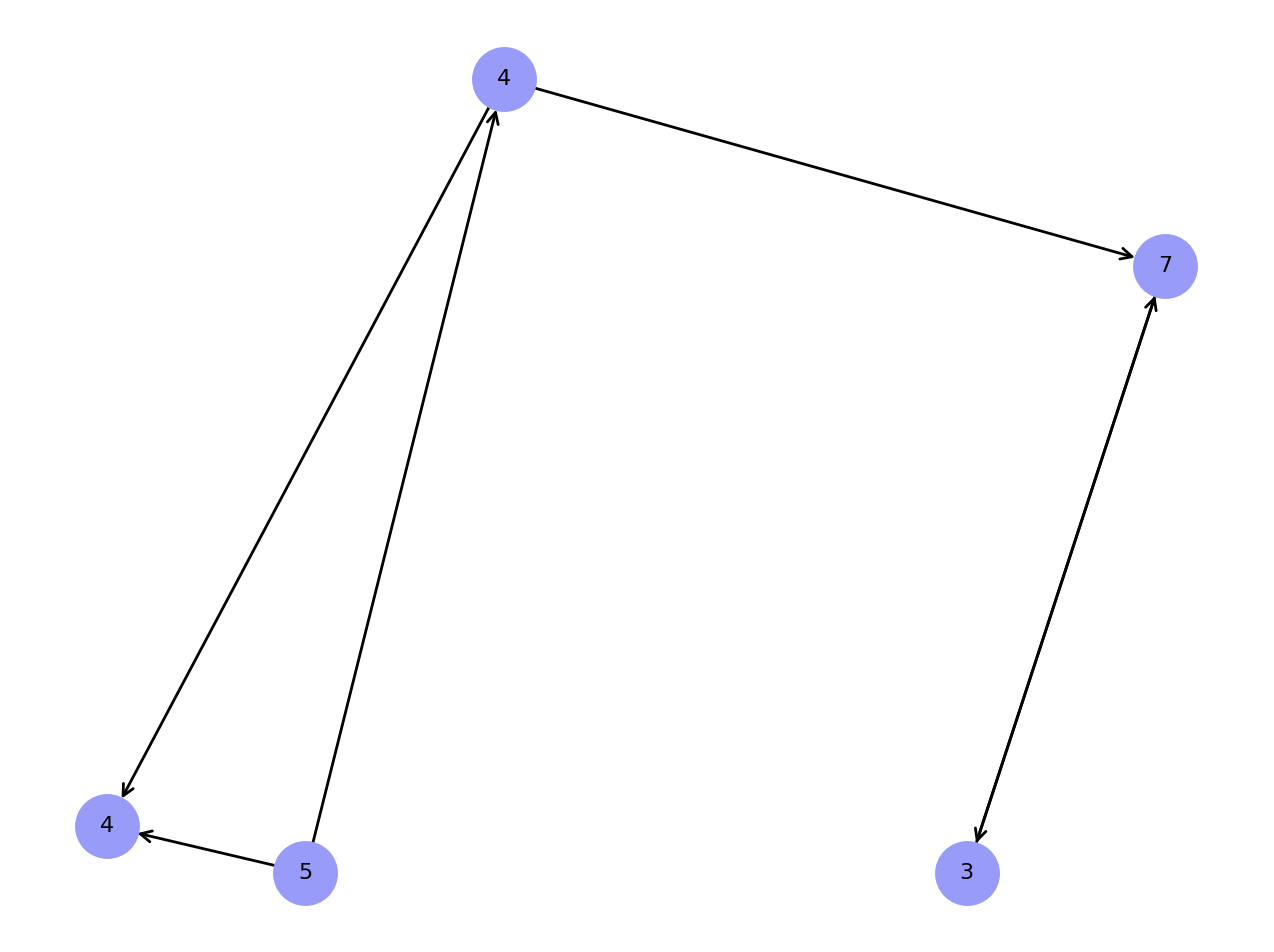
\includegraphics[width=0.8\columnwidth]{./figures/simple_graph.png}
    \caption{Example of a simple graph}
    \label{fig:Cloud Computing Types}
\end{figure}

The graph above has 5 sets that are closures:

\begin{itemize}
    \item 4 (weight: 4)
    \item 3, 7 (weight: 10)
    \item 3, 7, 4 (weight: 14)
    \item 3, 7, 4, 4 (weight: 18)
    \item 3, 7, 4, 4, 5 (whole graph) (weight: 23)
\end{itemize}

Therefore, the minimum weighted closure of this graph is 4, as it represents the minimum sum of closure vertices' weights.

\section{ Implementation Description}

To compute using both the exhaustive and the greedy search, there are two options to create a graph. A graph can be read from a file, with the following format

\begin{figure}[!htb]
    \centering
    \includegraphics[width=1\columnwidth]{./figures/usage.png}
    \caption{Main Program Usage}
    \label{fig:Program Usage}
\end{figure}


\begin{figure}[!htb]
    \centering
    \includegraphics[width=1\columnwidth]{./figures/example-solution-exhaustive.png}
    \caption{Example Exhaustive Solution found with Visualization tool}
    \label{fig: Example Solution}
\end{figure}


\begin{figure}[!htb]
    \centering
    \includegraphics[width=1\columnwidth]{./figures/example-solution-greedy.png}
    \caption{Example Exhaustive Solution found with Visualization tool}
    \label{fig: Example Solution}
\end{figure}



\subsection{Exhaustive Search}

\subsubsection{Formal Computational Complexity Analysis}


\subsection{Greedy Search}

\subsubsection{Formal Computational Complexity Analysis}



\section{Results and Discussion}


\begin{table}[!htb]
\resizebox{0.45 \textwidth}{!}{%
\begin{tabular}{||c c c c c||}
 \hline
 V & E & Operations  & Tested Sols. & Exec.Time(ms) \\ [0.2ex] 
 \hline\hline
 5 & 5 & 52 & 31 & 0.04 \\ 
 \hline
 7 & 13 & 166 & 127 & 0.19 \\
 \hline
 10 & 21 & 1234 & 1023 & 0.98\\
 \hline
 15 & 45 & 42924 & 32767 & 32.84 \\
 \hline
 17 & 41 & 141971 & 131071 & 108.18 \\
 \hline
 20 & 55 & 1624913 & 1048575 & 1250.05 \\
 \hline 
 25 & 131 & 33686474 & 33554431 & 33705.21 \\
 \hline 
 30 & 167 & 1576111704 & 1073741823 & 1910669.58 \\ [1ex] 
 \hline
\end{tabular}
%
}
\caption{\label{tab:table-name}Obtained results for the Exhaustive Approach}
\end{table}
 


\begin{figure}[!htb]
\flushleft
    \includegraphics[width=1\columnwidth]{./figures/results.png}
    \caption{Execution time(ms) in function of the Number of Vertices for the Exhaustive Approach}
    \label{fig: Example Solution}
\end{figure}


\begin{table}[!htb]
\resizebox{0.45 \textwidth}{!}{%
\begin{tabular}{||c c c c c||}
 \hline
 V & E & Operations  & Tested Sols. & Exec.Time(ms) \\ [0.2ex] 
 \hline\hline
 5 & 5 & 12 & 5 & 0.017 \\ 
 \hline
 7 & 13 & 18 & 7 & 0.019 \\
 \hline
 10 & 21 & 19 & 10 & 0.020 \\
 \hline
 15 & 45 & 42924 & 15 & 0.025 \\
 \hline
 17 & 41 & 44 & 17 &  0.035 \\
 \hline
 20 & 55 & 48 & 20 & 0.038 \\
 \hline 
 25 & 131 & 55 & 25 & 0.05 \\
 \hline 
 30 & 167 & 85 & 30 &  0.067 \\ 
 \hline 
... & ... & ... & ... & ... \\
 \hline 
 100 & 1772 & 199 & 100 &  0.303 \\[1ex] 
 \hline
\end{tabular}
%
}
\caption{\label{tab:table-name}Obtained results for the Greedy Approach}
\end{table}
 


\begin{figure}[!htb]
    \centering
    \includegraphics[width=1\columnwidth]{./figures/results2.png}
    \caption{Execution time in function of the Number of Vertices for the Greedy Approach}
    \label{fig: Example Solution}
\end{figure}


\section{Conclusion}


\begin{thebibliography}{9}

\bibitem{closure_problem}
Wikipedia contributors. (2020, November 25). Closure problem. Wikipedia. \url{https://en.wikipedia.org/wiki/Closure_problem}

\bibitem{Picard}
Picard, J. C. (1976). Maximal Closure of a Graph and Applications to Combinatorial Problems. Management Science, 22(11), 1268–1272. 
\url{https://doi.org/10.1287/mnsc.22.11.1268}
\end{thebibliography}




% use a field named url or \url{} for URLs
% Note: the \bibliographystyle is set automatically

\end{document}
